\documentclass[12pt,a4paper]{article}

\usepackage[utf8]{inputenc}
\usepackage[T1]{fontenc}
\usepackage[brazilian]{babel}
\usepackage{geometry}
\usepackage{graphicx}
\usepackage{booktabs}
\usepackage{longtable}
\usepackage{array}
\usepackage{float}
\usepackage{hyperref}
\usepackage{xcolor}
\usepackage{enumitem}
\usepackage{lmodern}

\geometry{margin=2.5cm}
\emergencystretch=3em
\setlength{\parindent}{1.25cm}
\setlength{\parskip}{0.15cm}
\setcounter{tocdepth}{2}
\renewcommand{\contentsname}{Sumário}
\setlist[itemize]{label=--, leftmargin=1.1cm}
\setlist[enumerate]{leftmargin=1.1cm}

\hypersetup{
    colorlinks=true,
    linkcolor=blue,
    urlcolor=blue
}
\setlength{\parindent}{1.25cm}
\begin{document}

\pagenumbering{gobble}
\begin{titlepage}
\centering

\vspace*{0.5cm}

\includegraphics[width=0.34\textwidth]{src/Logo_FGV_-_Fundação_Getulio_Vargas.png}

\vspace{1.2cm}
{\Large Fundação Getulio Vargas\par}
\vspace{0.25cm}
{\large Laboratório de Políticas Públicas\par}

\vfill

\vspace{0.8cm}
{\huge \textbf{Entre Elogios e Críticas}\par}
\vspace{0.35cm}
{\Large Segurança Presente como Política Pública: Avaliação de Percepções Digitais\par}

\vfill

\begin{flushleft}
\large
\textbf{Autoras e autores}\\[0.3cm]
Maria Eduarda Mesquita Magalh\~aes\\
Bianca Fialho Salgado Djelberian\\
Maria Teresa Mendes Madureira\\
Kayo Francisco da Silva\\
Sarah Ribeiro Lattouf\\[0.8cm]
\textbf{Professora}\\[0.3cm]
Katia Aiko Nishiyama Alves
\end{flushleft}

\vfill

{\large Rio de Janeiro\\Junho de 2026\par}

\end{titlepage}

\pagenumbering{arabic}

\tableofcontents
\newpage

\section{Introdução}

O presente relatório sistematiza a etapa final de uma pesquisa voltada à aplicação de modelos de linguagem de grande escala na análise de notícias sobre políticas públicas de segurança. O objeto empírico é a cobertura jornalística online relativa ao programa Segurança Presente, iniciativa de policiamento de proximidade e ordenamento urbano associada ao Governo do Estado do Rio de Janeiro.

A motivação do estudo decorre de um problema metodológico recorrente em pesquisas sobre mídia e políticas públicas: a impossibilidade prática de classificar manualmente, com regularidade e escala, um conjunto amplo de textos jornalísticos. No caso de políticas de segurança, essa dificuldade é intensificada pela natureza heterogênea das notícias. Uma mesma base pode conter inaugurações de unidades, prisões, eventos culturais, críticas administrativas, denúncias, mudanças institucionais, estatísticas de criminalidade e menções laterais ao programa. Classificar esse material exige distinguir não apenas o tema geral da notícia, mas a forma como o programa é retratado em cada contexto.

O estudo, portanto, não mede opinião pública direta. A unidade de análise é a notícia publicada em ambiente digital. A inferência produzida refere-se à percepção retratada pela cobertura midiática, isto é, ao modo como o programa, seus agentes, sua gestão ou eventos relacionados aparecem nos textos analisados. Essa distinção é central: uma cobertura predominantemente positiva não equivale necessariamente a aprovação social majoritária, mas sinaliza que, no corpus examinado, as notícias tendem a enquadrar o programa em termos favoráveis, operacionais, institucionais ou de reforço de presença estatal.

\section{Problema de pesquisa}

A pergunta que orientou a implementação foi: de que modo um modelo de linguagem de grande escala pode classificar notícias sobre o Segurança Presente quanto ao sentimento retratado e ao evento factual central mencionado em cada texto?

Essa pergunta foi traduzida em três desafios operacionais. O primeiro consistiu em definir critérios de pertinência temática, para que apenas notícias com menção substantiva ao programa fossem classificadas. O segundo consistiu em converter textos jornalísticos não estruturados em variáveis analíticas comparáveis, como classe de sentimento, escore numérico, tipo de evento e localidade. O terceiro consistiu em agregar resultados individuais em tabelas, gráficos e rankings capazes de apoiar interpretação substantiva sobre padrões da cobertura.

\section{Objetivos}

\subsection{Objetivo geral}

Construir e documentar um procedimento automatizado, reprodutível e tecnicamente transparente para classificar notícias sobre o programa Segurança Presente, combinando análise de sentimento, extração de eventos e produção de indicadores descritivos sobre a cobertura jornalística.

\subsection{Objetivos específicos}

\begin{enumerate}
    \item Consolidar uma base jornalística obtida por webscrapping e transformá-la em registros textuais padronizados.
    \item Aplicar um filtro de pertinência que mantenha somente notícias com ocorrência explícita da expressão ``Segurança Presente''.
    \item Classificar cada notícia segundo uma escala ordinal de sentimento.
    \item Converter os rótulos de sentimento em escores numéricos comparáveis.
    \item Identificar o evento factual central de cada notícia, evitando categorias genéricas.
    \item Remover duplicatas antes das análises agregadas, preservando a rastreabilidade da base bruta.
    \item Produzir estatísticas gerais, séries temporais, distribuição por fonte e rankings de eventos.
\end{enumerate}

\section{Dados e recorte empírico}

\subsection{Origem e natureza da base}

A base empírica foi formada por notícias coletadas por webscrapping em veículos digitais, portais de notícias, sites institucionais e páginas jornalísticas que continham material relacionado ao Segurança Presente. Cada registro coletado preservou, quando disponível, título, resumo, corpo textual, fonte de publicação, endereço de origem, data de publicação, identificadores internos e metadados de agrupamento.

Por se tratar de uma base derivada de coleta automatizada na web, os registros apresentam variação de completude. O procedimento metodológico foi desenhado para lidar com essa heterogeneidade sem descartar automaticamente notícias apenas por ausência de corpo integral, desde que houvesse informação textual suficiente para classificação.

\subsection{Filtro de pertinência temática}

Antes da classificação por modelo de linguagem, aplicou-se um filtro textual estrito. O procedimento combinou título, resumo e texto bruto de cada notícia, normalizou acentos e caixa, e manteve apenas registros que continham a expressão exata ``Segurança Presente''. Essa escolha reduziu o risco de classificar notícias de segurança pública que não tratavam diretamente do programa.

\subsection{Tamanho da base}

\begin{table}[H]
\centering
\begin{tabular}{p{10cm}r}
\toprule
\textbf{Etapa metodológica} & \textbf{Quantidade} \\
\midrule
Registros jornalísticos brutos obtidos por webscrapping & 863 \\
Registros mantidos após o filtro explícito de ``Segurança Presente'' & 858 \\
Notícias únicas após deduplicação por identificador jornalístico & 847 \\
Notícias com data válida na base analítica final & 822 \\
\bottomrule
\end{tabular}
\caption{Dimensão da base em cada etapa do tratamento dos dados.}
\end{table}

\subsection{Cobertura temporal}

Entre as notícias com data válida, o período observado vai de 31 de maio de 2016 a 11 de junho de 2026. As notícias sem data válida foram preservadas em análises gerais, mas excluídas das visualizações temporais, pois não poderiam ser corretamente posicionadas em séries mensais.

\section{Desenho metodológico}

Primeiro, os dados brutos foram carregados e convertidos em observações padronizadas. Em seguida, cada notícia passou por filtragem temática, composição textual, classificação automatizada, validação dos rótulos retornados, deduplicação, agregação estatística e organização dos resultados finais.

A opção por um fluxo sequencial teve finalidade metodológica: permitir que cada etapa produzisse um artefato analítico verificável, ao mesmo tempo em que preservava a rastreabilidade entre o registro bruto e a notícia classificada. Assim, a pesquisa não se limitou a solicitar respostas individuais a um modelo de linguagem; ela construiu uma cadeia de tratamento dos dados capaz de gerar resultados consistentes e replicáveis.

\subsection{Padronização dos registros}

Cada notícia foi convertida em uma observação analítica contendo identificador, ordem de ocorrência na base, título, fonte, data, resumo, texto bruto e metadados de origem. Essa padronização foi necessária porque os textos coletados por webscrapping não possuem estrutura uniforme. A normalização permitiu tratar registros completos e incompletos dentro de um mesmo protocolo de análise.

Para fins de classificação, foi formado um campo textual composto pela concatenação do título, do resumo e do corpo da notícia. A criação desse campo reduz perda de informação quando o texto integral está ausente, pois o título e o resumo frequentemente contêm a pauta central da notícia. Ao mesmo tempo, quando o corpo integral existe, ele amplia a base de evidências disponível para o modelo.

\section{Classificação automatizada}

\subsection{Modelo e parâmetros}

A classificação foi realizada com o modelo \texttt{gpt-4o-mini}, da família GPT, configurado para operar com temperatura zero. O uso de temperatura zero buscou reduzir variações aleatórias entre chamadas e tornar as respostas mais estáveis. Cada requisição solicitou uma saída estruturada em formato JSON, o que possibilitou posterior leitura automatizada, validação de campos e agregação tabular.


\subsection{Prompt analítico}

O instrumento central da classificação foi um prompt único, desenhado para executar simultaneamente duas tarefas: classificar o sentimento retratado na notícia e extrair o evento factual central. A decisão de usar um único prompt foi metodologicamente relevante, pois sentimento e evento são dimensões interdependentes. A interpretação de uma notícia sobre inauguração, prisão, denúncia ou grande evento público depende do acontecimento específico a que ela se refere.

O prompt determinou que o sentimento deveria se referir ao modo como o programa, sua gestão, seus agentes ou eventos diretamente relacionados eram retratados. Assim, crimes não foram automaticamente classificados como negativos e prisões não foram automaticamente classificadas como positivas; em ambos os casos, era necessário que o texto associasse o acontecimento ao programa de forma substantiva.

Além disso, o prompt exigiu a identificação de um evento específico. Categorias amplas, como ``segurança pública'', ``policiamento'' ou ``violência urbana'', foram consideradas insuficientes. O evento deveria ser concreto o bastante para distinguir acontecimentos diferentes, mas estável o bastante para agrupar notícias sobre o mesmo fato.

\subsection{Variáveis extraídas}

A classificação produziu um conjunto de variáveis analíticas. A primeira corresponde ao rótulo de sentimento, que sintetiza a percepção retratada. A segunda é um escore numérico associado ao rótulo, utilizado para cálculo de médias e rankings. O procedimento também extraiu uma justificativa curta, uma descrição do evento principal, uma chave canônica para agrupamento, o tipo de evento, local, data quando disponível e evidências textuais ou paráfrases fiéis que sustentam a decisão.

Esses campos não foram tratados como simples metadados técnicos. Eles funcionam como ponte entre leitura qualitativa e mensuração quantitativa. A justificativa e as evidências permitem revisão humana; o escore e a chave de evento permitem agregação estatística.

\section{Escala de sentimento}

O sentimento foi classificado em seis categorias mutuamente exclusivas: muito negativo, negativo, neutro, positivo, muito positivo e não aplicável. A classe não aplicável foi reservada para notícias que mencionavam o Segurança Presente de forma lateral ou sem elementos suficientes para avaliar o programa, seus agentes, sua gestão ou evento diretamente relacionado.

\begin{table}[H]
\centering
\begin{tabular}{p{4cm}rp{8cm}}
\toprule
\textbf{Categoria} & \textbf{Escore} & \textbf{Interpretação operacional} \\
\midrule
Muito negativo & -2 & Retrato de falha grave, crise, violência severa, ilegalidade, denúncia robusta ou dano institucional associado ao programa. \\
Negativo & -1 & Cobertura marcada por crítica, controvérsia, problema operacional, insegurança, limitação ou efeito desfavorável. \\
Neutro & 0 & Notícia predominantemente informativa, administrativa ou descritiva, sem avaliação clara. \\
Positivo & 1 & Retrato de expansão, inauguração, reforço, operação, resultado favorável, prisão, apreensão ou apoio institucional associado ao programa. \\
Muito positivo & 2 & Resultado excepcional, reconhecimento expressivo, forte celebração institucional ou impacto favorável de grande magnitude. \\
Não aplicável & -- & Menção lateral ou insuficiente, sem base textual para inferir percepção sobre o programa ou evento relacionado. \\
\bottomrule
\end{tabular}
\caption{Escala de sentimento e conversão em escore numérico.}
\end{table}

A conversão para escore não transforma a classificação em medida causal ou psicológica. Ela oferece apenas uma escala ordinal simplificada para comparar agregados, calcular médias por evento e ordenar grupos de notícias segundo a direção predominante da cobertura.

\section{Agregação e produtos analíticos}

Após a deduplicação, a base analítica foi usada para produzir quatro grupos de resultados. O primeiro grupo contém a classificação individual de cada notícia única. O segundo reúne tabelas de distribuição geral, distribuição mensal e fontes. O terceiro reúne gráficos descritivos, incluindo barras de sentimento, histograma de escore, evolução mensal dos percentuais, volume mensal de notícias e distribuição por fonte. O quarto grupo contém o ranqueamento de eventos, calculado a partir da chave canônica extraída pelo modelo.

Os gráficos foram selecionados para responder a perguntas complementares. A distribuição geral indica a composição agregada do corpus. As séries temporais mostram variações no tempo. A análise por fonte permite observar concentração de cobertura em determinados veículos. O ranking de eventos desloca a análise do nível geral para acontecimentos concretos.

\section{Resultados descritivos}

\subsection{Distribuição geral dos sentimentos}

\begin{table}[H]
\centering
\begin{tabular}{lrr}
\toprule
\textbf{Sentimento} & \textbf{Notícias} & \textbf{Percentual} \\
\midrule
Muito negativo & 27 & 3,19\% \\
Negativo & 189 & 22,31\% \\
Neutro & 21 & 2,48\% \\
Positivo & 512 & 60,45\% \\
Muito positivo & 2 & 0,24\% \\
Não aplicável & 96 & 11,33\% \\
\bottomrule
\end{tabular}
\caption{Distribuição de sentimentos na base final deduplicada.}
\end{table}

Os resultados indicam predominância de notícias classificadas como positivas. Somadas, as categorias positiva e muito positiva representam 514 notícias, equivalentes a 60,69\% da base final. As categorias negativa e muito negativa somam 216 notícias, ou 25,50\% do total. A classe não aplicável representa 11,33\%, o que revela a presença de menções laterais ou pouco informativas sobre o programa mesmo após o filtro textual.

Esse padrão sugere que, no corpus analisado, o Segurança Presente é frequentemente retratado em notícias sobre expansão, inauguração de bases, reforço de policiamento, organização de eventos, prisões, apreensões e ações de presença estatal. Entretanto, o volume de notícias negativas não é residual, indicando a existência de controvérsias, críticas e episódios desfavoráveis relevantes.

\subsection{Fontes de publicação}

A cobertura concentrou-se em um conjunto relativamente pequeno de fontes. As dez fontes com maior volume responderam por parcela expressiva do corpus, com destaque para portais regionais e veículos digitais voltados à cobertura do Rio de Janeiro. A concentração por fonte é relevante porque a composição do corpus pode influenciar a distribuição de sentimentos: veículos institucionais, portais locais e sites noticiosos podem ter padrões distintos de seleção, enquadramento e reprodução de releases.

\begin{table}[H]
\centering
\begin{tabular}{lr}
\toprule
\textbf{Fonte} & \textbf{Notícias} \\
\midrule
diariodorio.com & 452 \\
agendadopoder.com.br & 123 \\
temporealrj.com & 119 \\
tribunadaserra.com.br & 38 \\
vejario.abril.com.br & 22 \\
oglobo.globo.com & 17 \\
g1.globo.com & 8 \\
voltaredonda.rj.gov.br & 8 \\
buzios.rj.gov.br & 7 \\
ssp.am.gov.br & 6 \\
\bottomrule
\end{tabular}
\caption{Principais fontes presentes na base analítica final.}
\end{table}

\section{Ranking de eventos}

\subsection{Critério de construção}

O ranking de eventos foi construído a partir da chave canônica atribuída pelo modelo de linguagem a cada notícia. Para cada evento, foram calculados o número de notícias associadas, a quantidade de notícias com escore válido, a média do escore de sentimento, a proporção de notícias positivas, a proporção de notícias negativas e a distribuição dos rótulos individuais.

Para reduzir instabilidade estatística, o ranking principal considerou apenas eventos com pelo menos três notícias. Esse critério impede que um evento mencionado uma única vez apareça no topo ou na base do ranking apenas por ter recebido classificação extrema. A ordenação dos eventos mais positivamente retratados priorizou maior escore médio, maior proporção de notícias positivas, maior peso de classificações muito positivas e maior número de notícias. A ordenação dos eventos mais negativamente retratados aplicou lógica inversa, priorizando menor escore médio, maior proporção de negativas, maior peso de classificações muito negativas e maior número de notícias.

Para apresentação no relatório, o escore médio original, definido na escala de -2 a 2, foi normalizado para o intervalo de 0 a 1. A transformação aplicada foi:

\[
\text{SCOREnormalizado} = \frac{\text{SCOREmédio} + 2}{4}
\]

Com isso, valores próximos de 0 indicam cobertura fortemente negativa, valores próximos de 0,5 indicam neutralidade ou equilíbrio e valores próximos de 1 indicam cobertura fortemente positiva. A normalização altera apenas a escala de apresentação; ela não modifica a ordenação substantiva dos rankings.

\subsection{Eventos mais positivamente retratados}

\begin{longtable}{p{7.2cm}rrrr}
\toprule
\textbf{Evento} & \textbf{N} & \textbf{Score norm.} & \textbf{Positivas} & \textbf{Negativas} \\
\midrule
\endhead
Criação de comitê permanente de segurança escolar no Rio em 2023 & 4 & 0,7500 & 100,00\% & 0,00\% \\
Inauguração da base do Segurança Presente em Irajá em 2025 & 3 & 0,7500 & 100,00\% & 0,00\% \\
Lançamento da base do Segurança Presente em Búzios em 2025 & 3 & 0,7500 & 100,00\% & 0,00\% \\
Abertura de inscrições para o vestibular Cederj de 2026 & 3 & 0,7500 & 33,33\% & 0,00\% \\
Show da Shakira em Copacabana em 2026 & 4 & 0,7500 & 25,00\% & 0,00\% \\
\bottomrule
\caption{Top 5 eventos mais positivamente retratados, considerando apenas eventos com pelo menos três notícias e score normalizado em escala de 0 a 1.}
\end{longtable}

O topo do ranking positivo é composto por eventos administrativos, inaugurações, lançamentos de bases, ações de organização institucional e operações associadas a grandes eventos públicos. Esse resultado sugere que a cobertura tende a retratar o programa de forma favorável quando a pauta enfatiza expansão territorial, reforço operacional, presença estatal ou capacidade de organização em contextos de grande circulação de pessoas.

A presença de eventos com baixa proporção de notícias explicitamente positivas, mas escore médio elevado, indica que parte dos agrupamentos contém notícias classificadas como não aplicáveis ou neutras. Nesses casos, o escore médio é calculado apenas sobre classificações válidas, razão pela qual a interpretação deve considerar simultaneamente média, proporção de positivas e número total de notícias.

\subsection{Eventos mais negativamente retratados}

\begin{longtable}{p{7.2cm}rrrr}
\toprule
\textbf{Evento} & \textbf{N} & \textbf{Score norm.} & \textbf{Positivas} & \textbf{Negativas} \\
\midrule
\endhead
Desaparecimento de José Carlos Simonin em Copacabana em 2026 & 3 & 0,1667 & 0,00\% & 100,00\% \\
Inauguração da base do Segurança Presente em Iguaba Grande em 2026 & 3 & 0,4167 & 33,33\% & 66,67\% \\
Transferência do Segurança Presente para a Polícia Militar em 2026 & 3 & 0,5000 & 33,33\% & 33,33\% \\
Transferência do Segurança Presente para a Polícia Militar & 5 & 0,6250 & 40,00\% & 0,00\% \\
\bottomrule
\caption{Eventos mais negativamente retratados, considerando apenas eventos com pelo menos três notícias, ao menos uma notícia negativa e score normalizado em escala de 0 a 1.}
\end{longtable}

O evento mais negativamente retratado foi o desaparecimento de José Carlos Simonin em Copacabana em 2026, com score normalizado de 0,1667 e 100\% das notícias classificadas como negativas. Em seguida aparece o agrupamento relacionado à inauguração da base de Iguaba Grande, cujo score normalizado de 0,4167 decorre da mistura entre notícias de inauguração e textos associados a controvérsias administrativas. Esse caso evidencia uma limitação importante da extração automatizada de eventos: quando pautas próximas aparecem em um mesmo conjunto textual, o agrupamento pode reunir sinais substantivos distintos e demandar revisão qualitativa.

\section{Visualizações produzidas}

\subsection{Distribuição geral}

\begin{figure}[H]
\centering
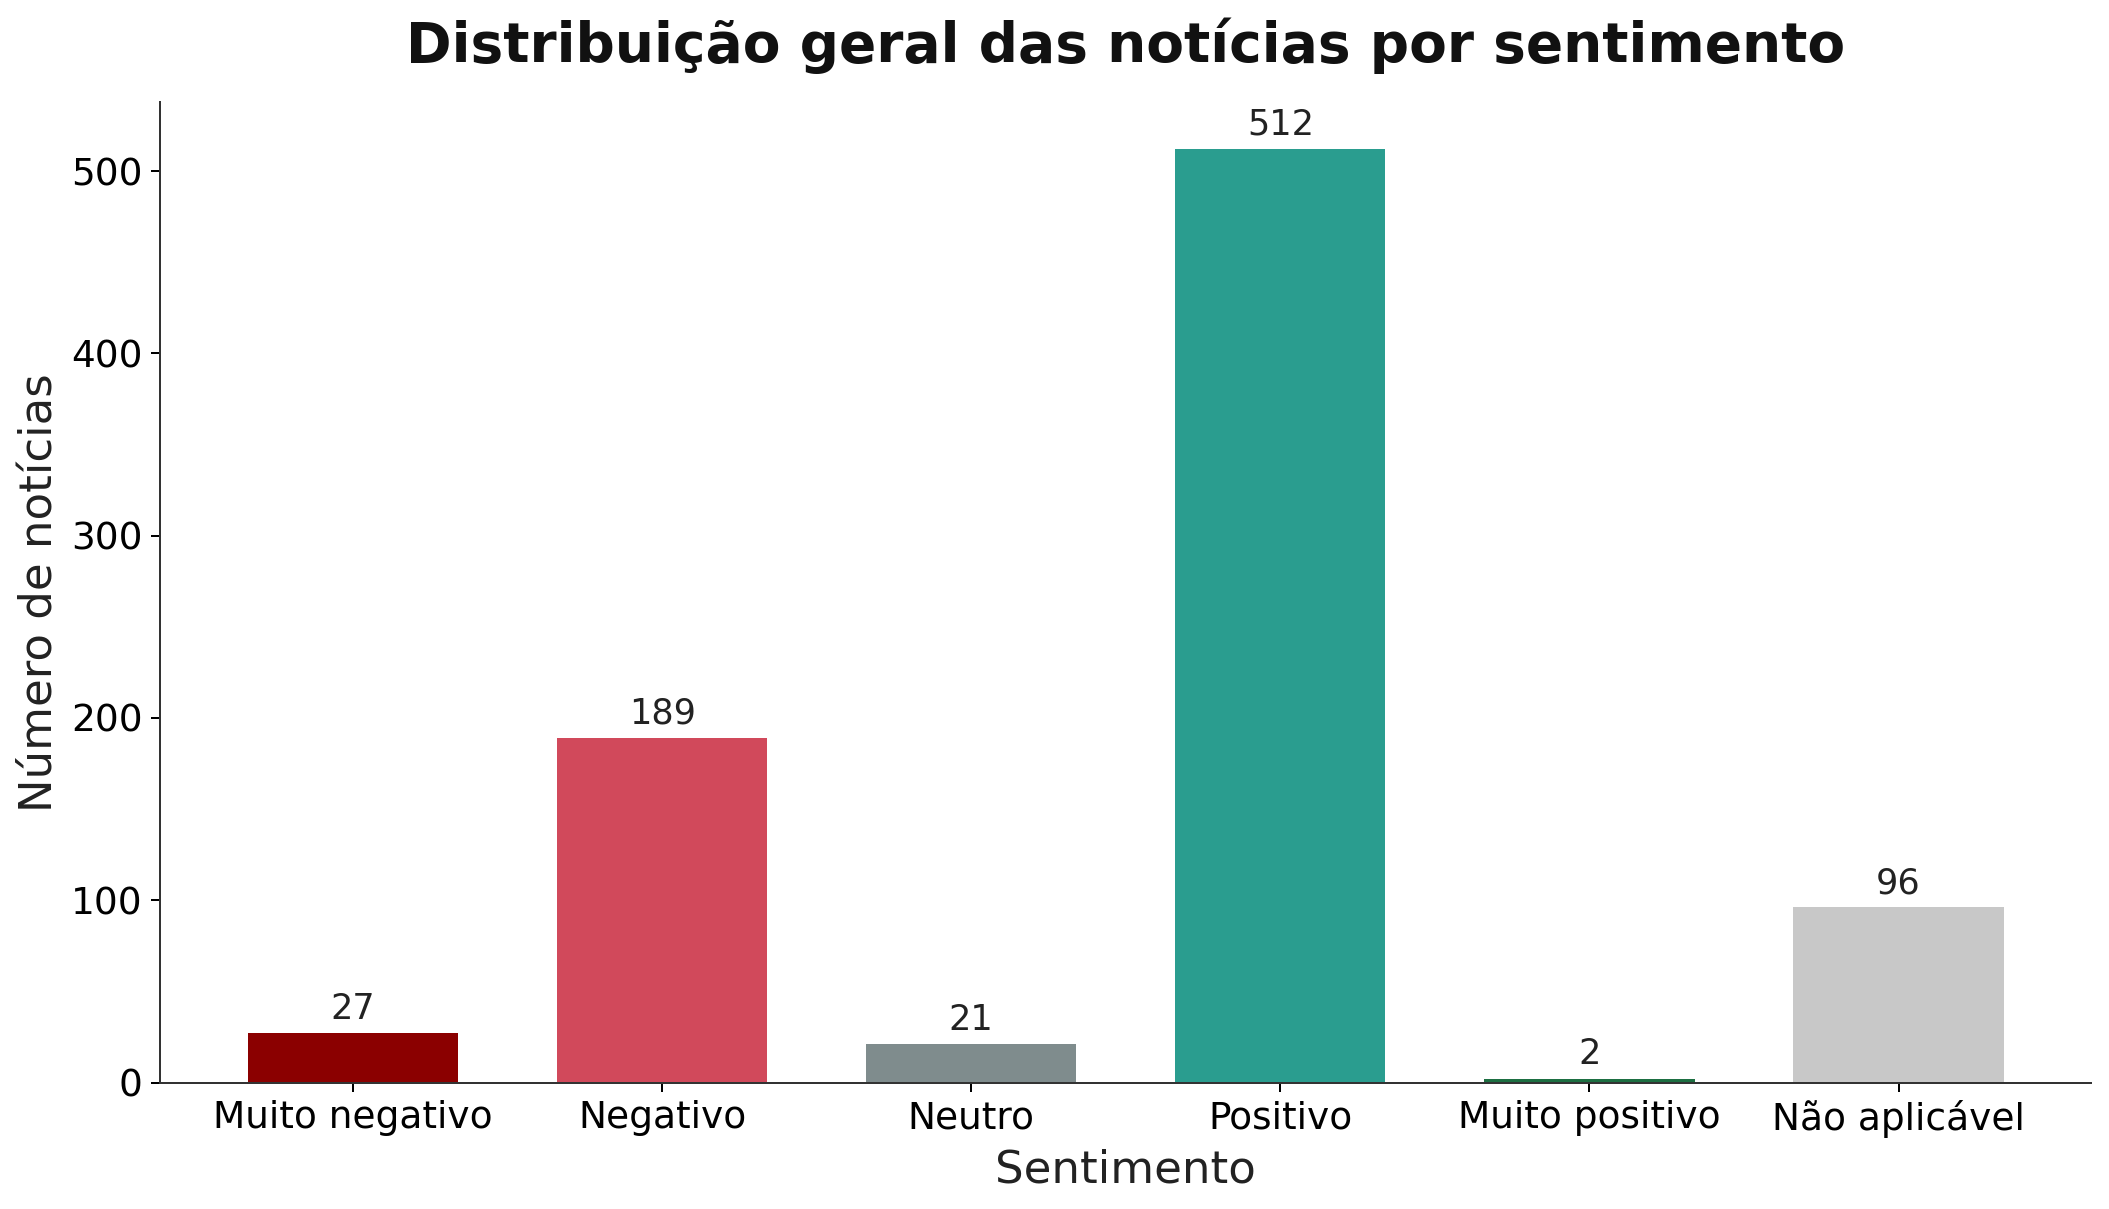
\includegraphics[width=0.9\textwidth]{graficos/barras_quantidade_por_sentimento.png}
\caption{Quantidade de notícias por sentimento.}
\end{figure}

\begin{figure}[H]
\centering
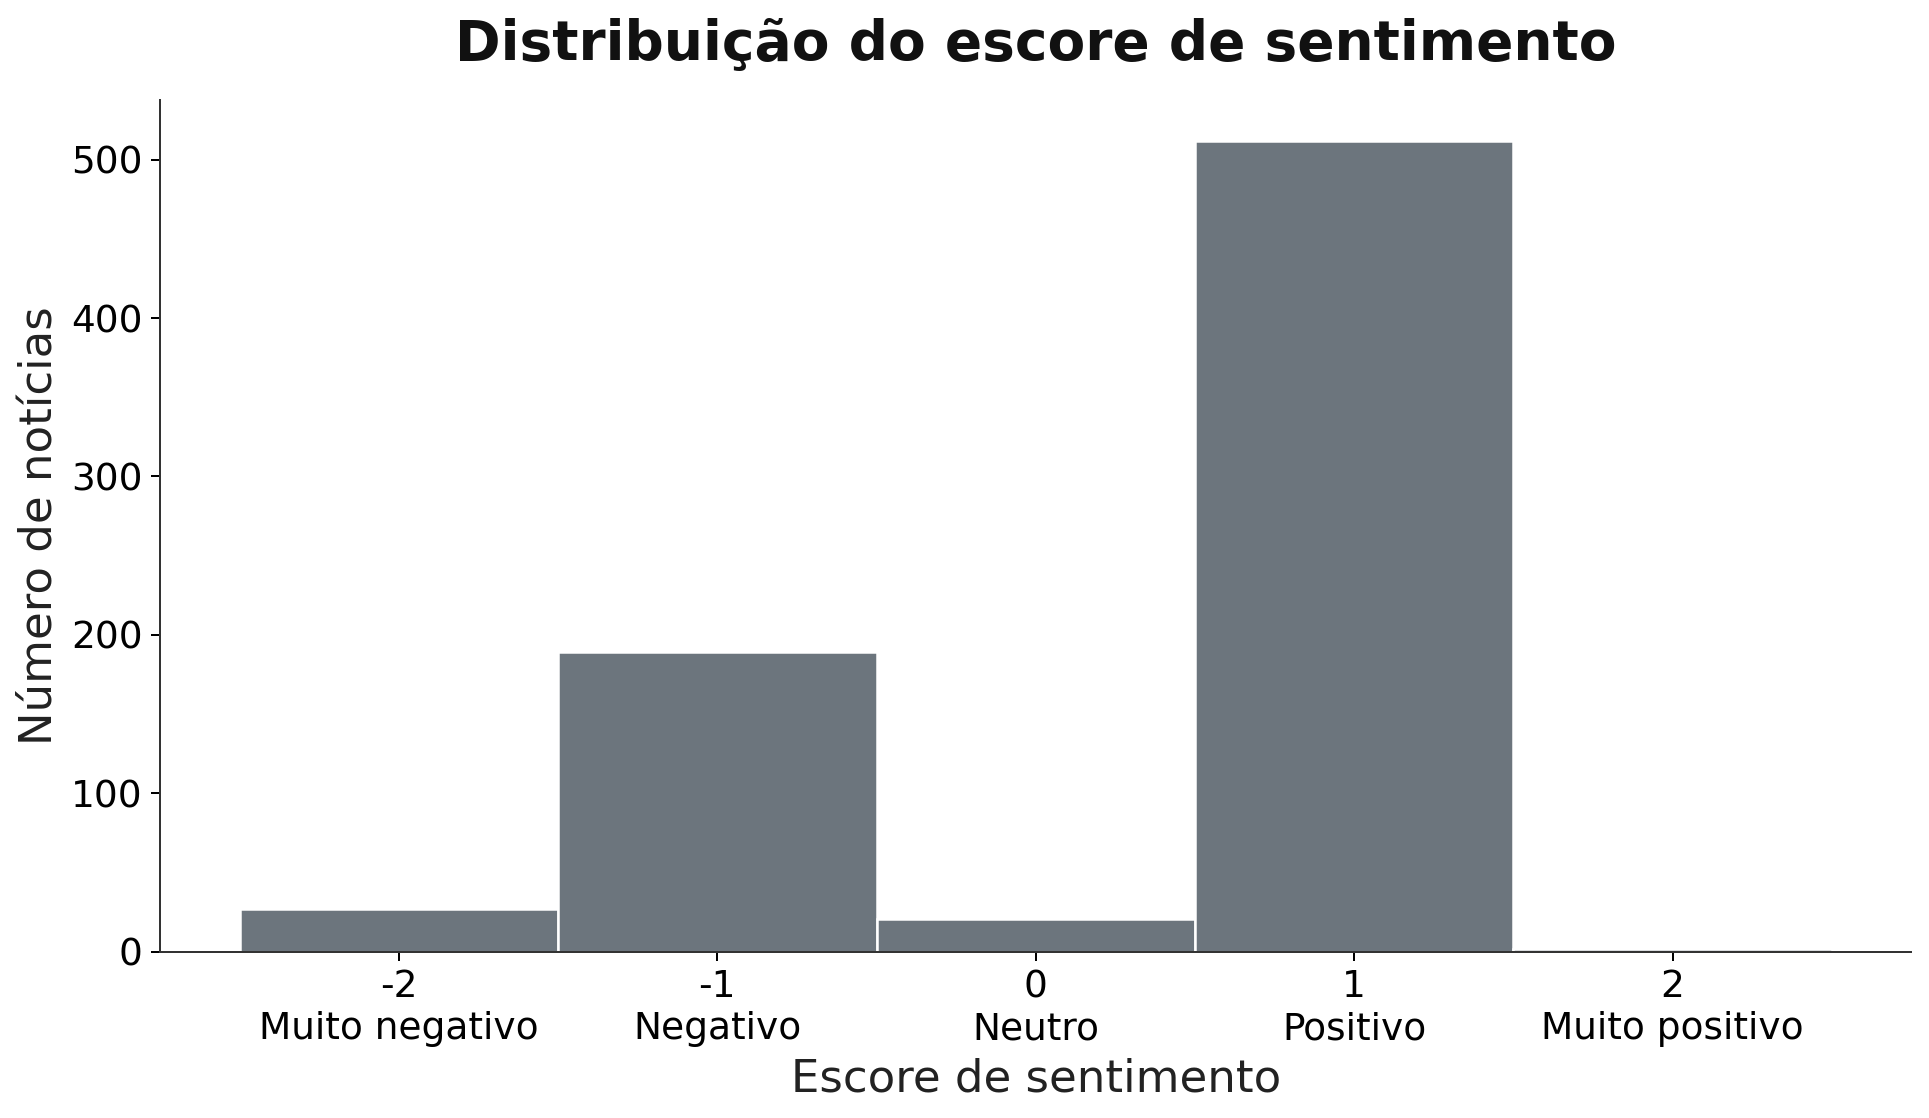
\includegraphics[width=0.9\textwidth]{graficos/histograma_escore_sentimento.png}
\caption{Histograma do escore de sentimento.}
\end{figure}

\subsection{Evolução temporal}

\begin{figure}[H]
\centering
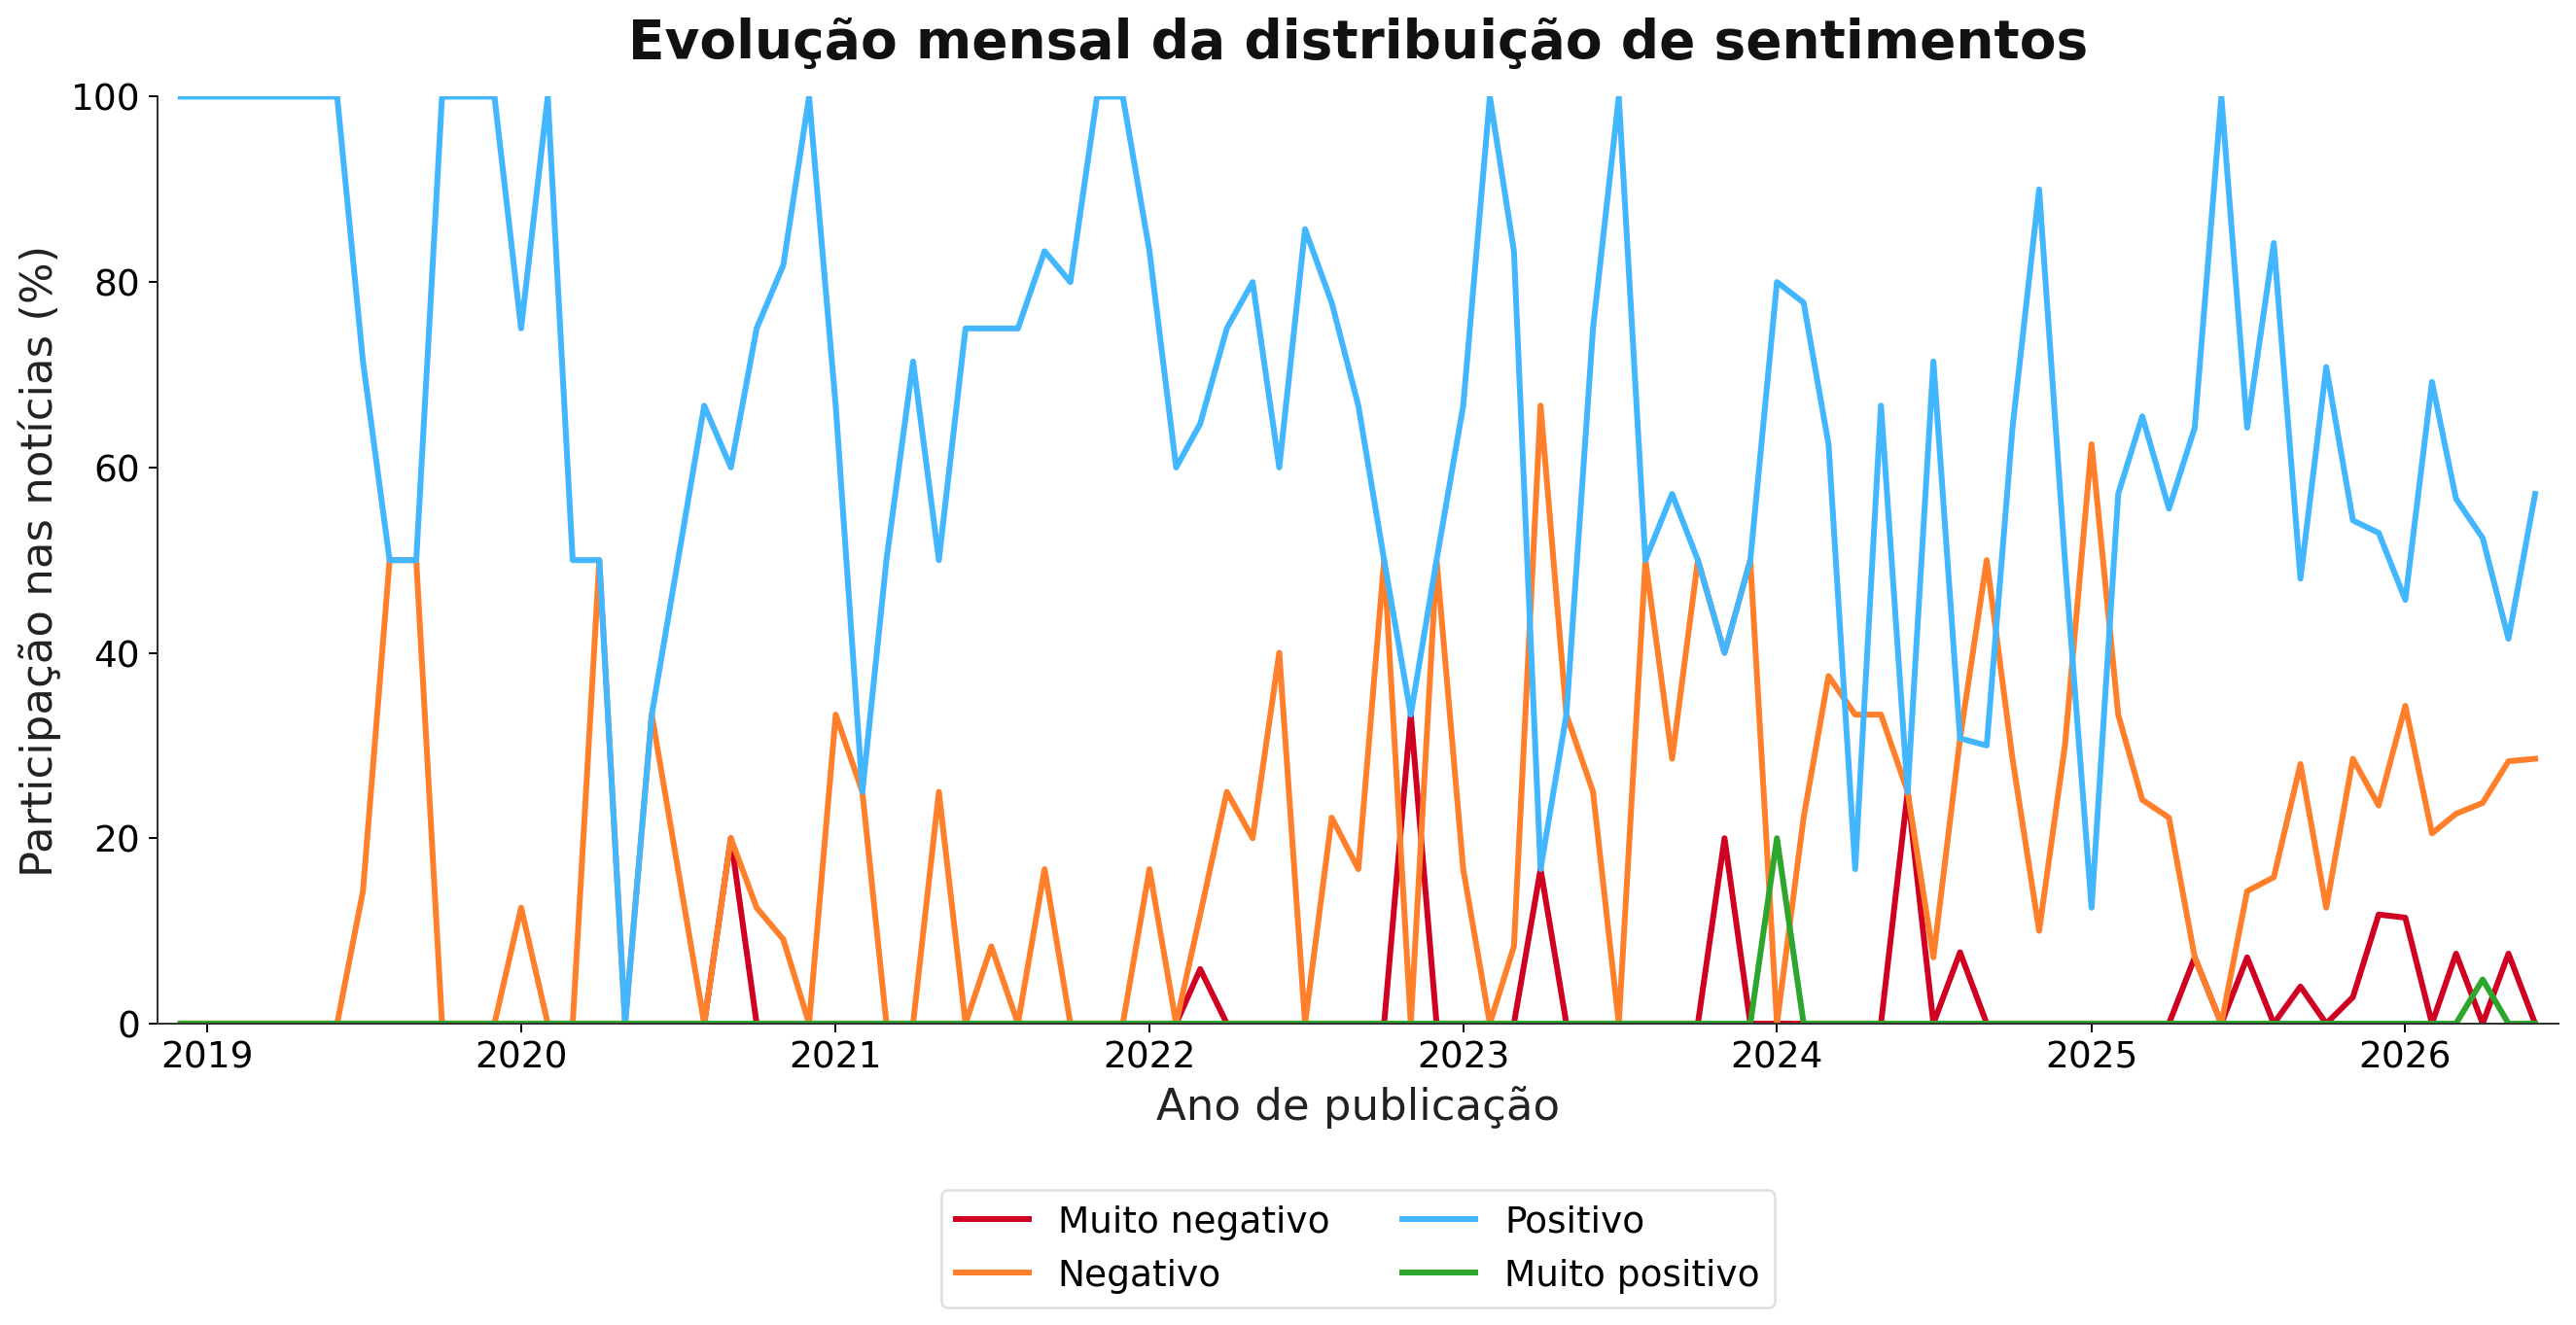
\includegraphics[width=0.95\textwidth]{graficos/linha_percentual_mensal_sentimentos.png}
\caption{Percentual mensal de notícias por sentimento.}
\end{figure}

\begin{figure}[H]
\centering
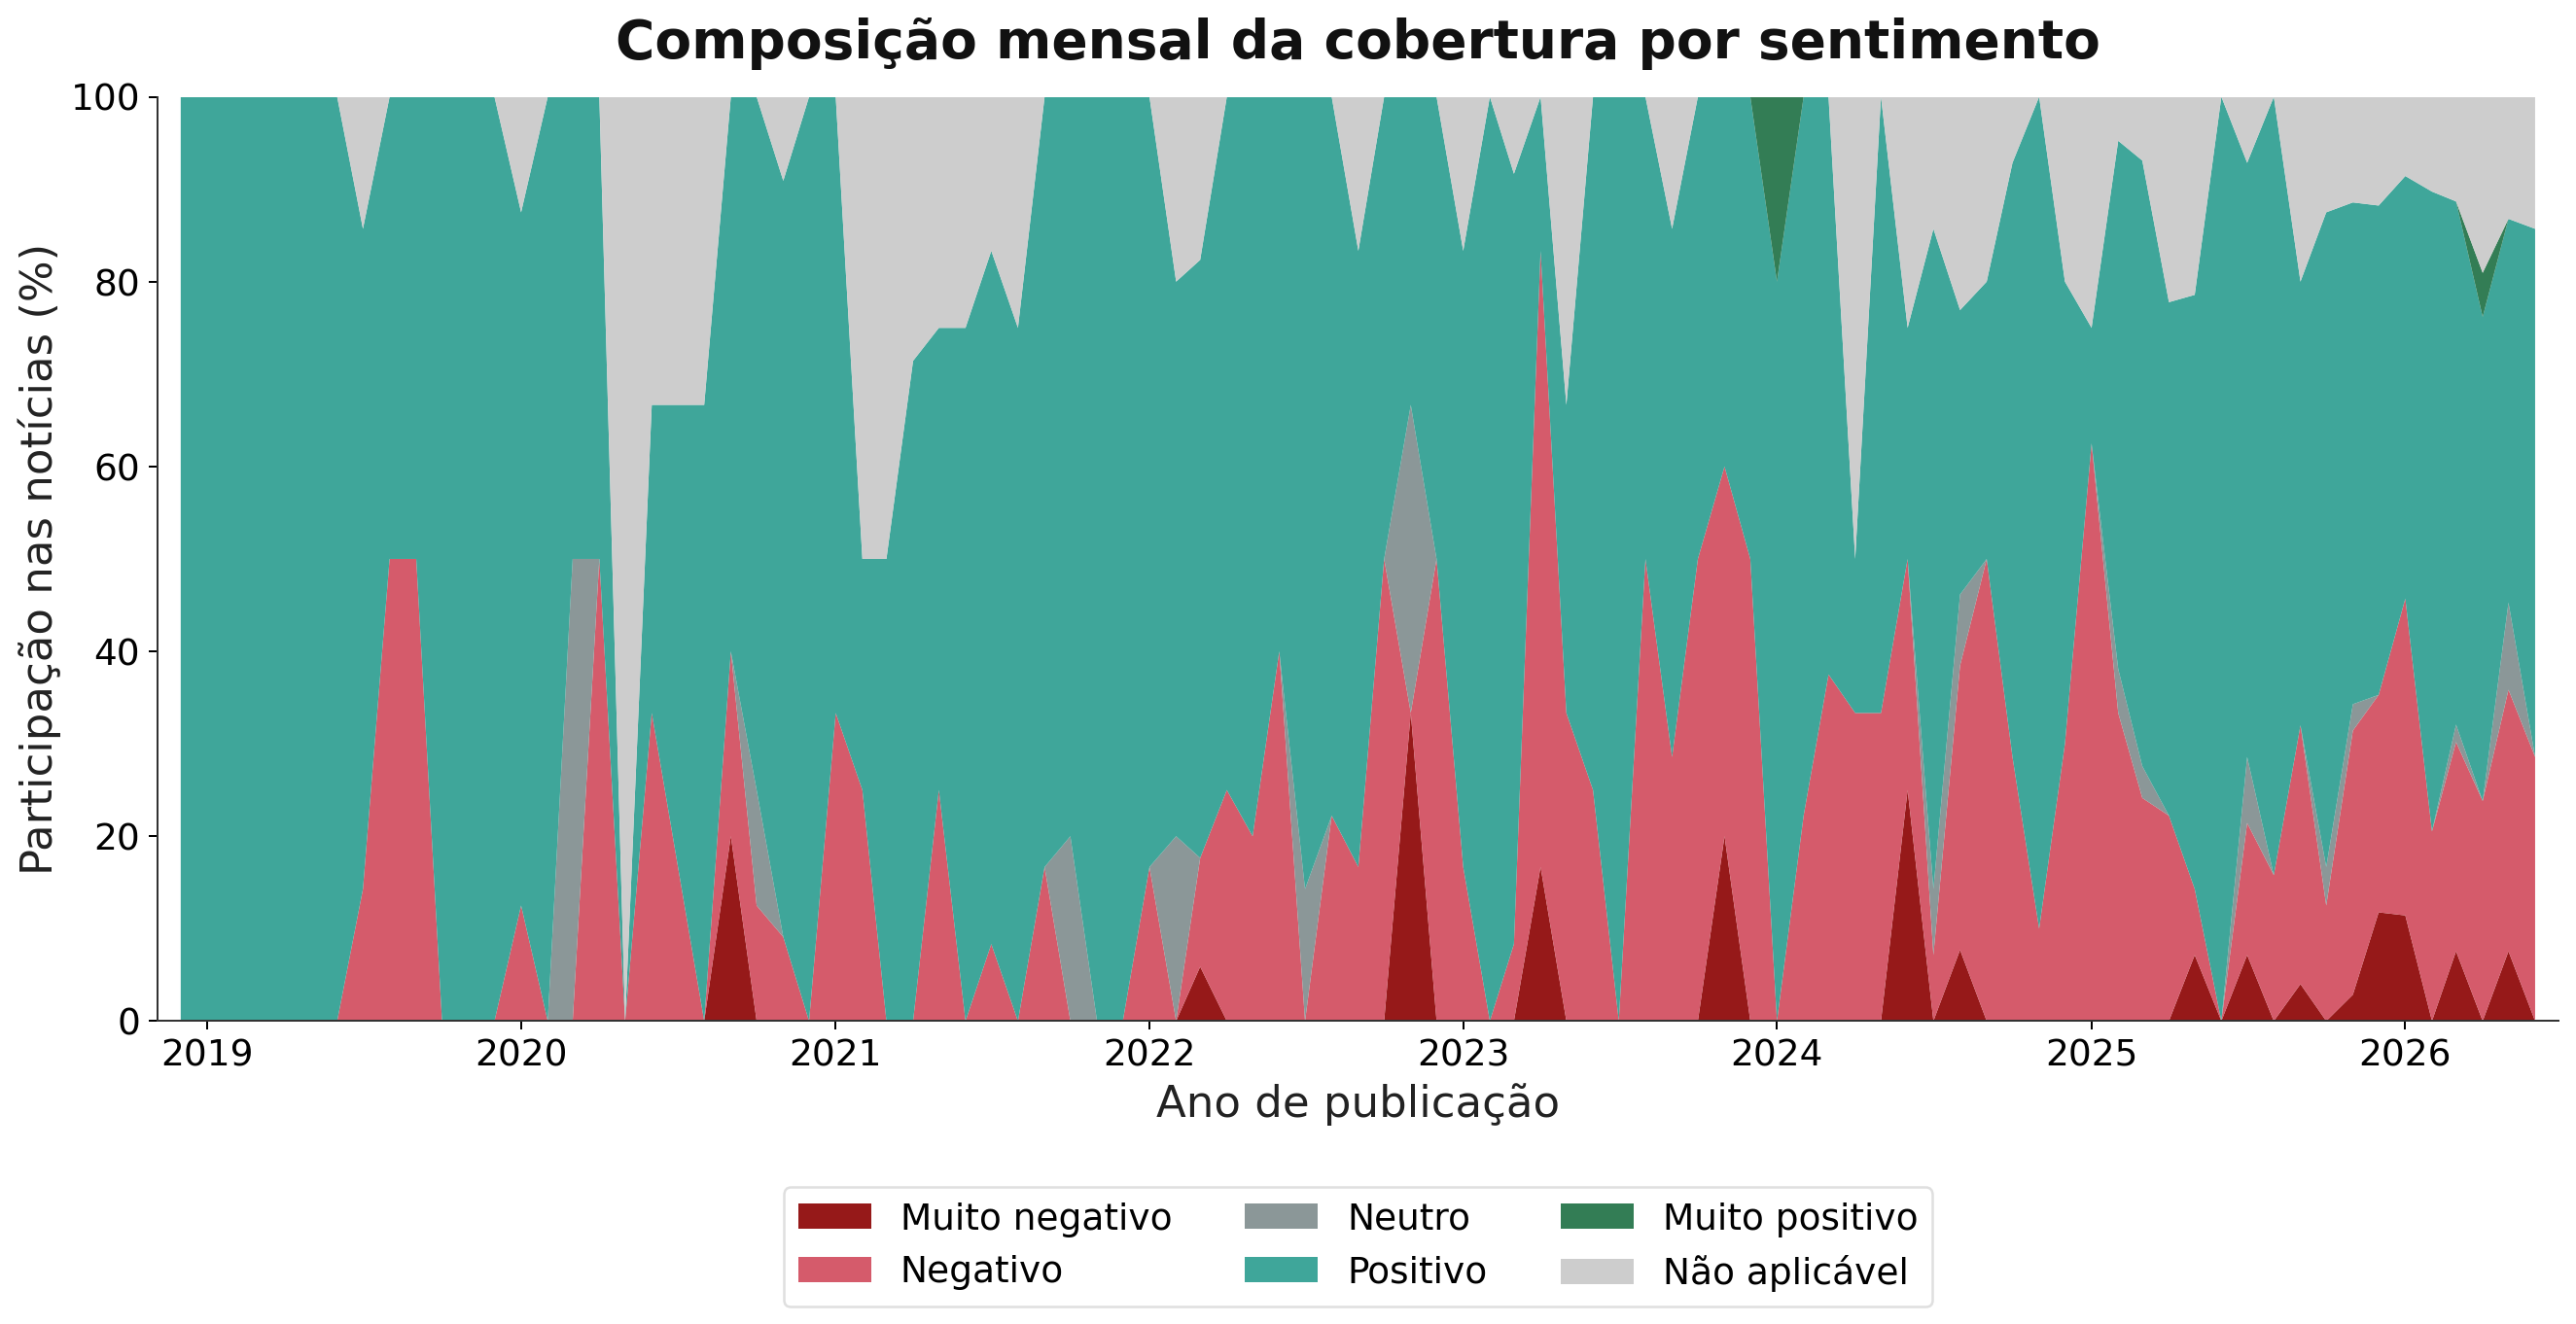
\includegraphics[width=0.95\textwidth]{graficos/area_empilhada_percentual_mensal.png}
\caption{Composição mensal dos sentimentos.}
\end{figure}

\begin{figure}[H]
\centering
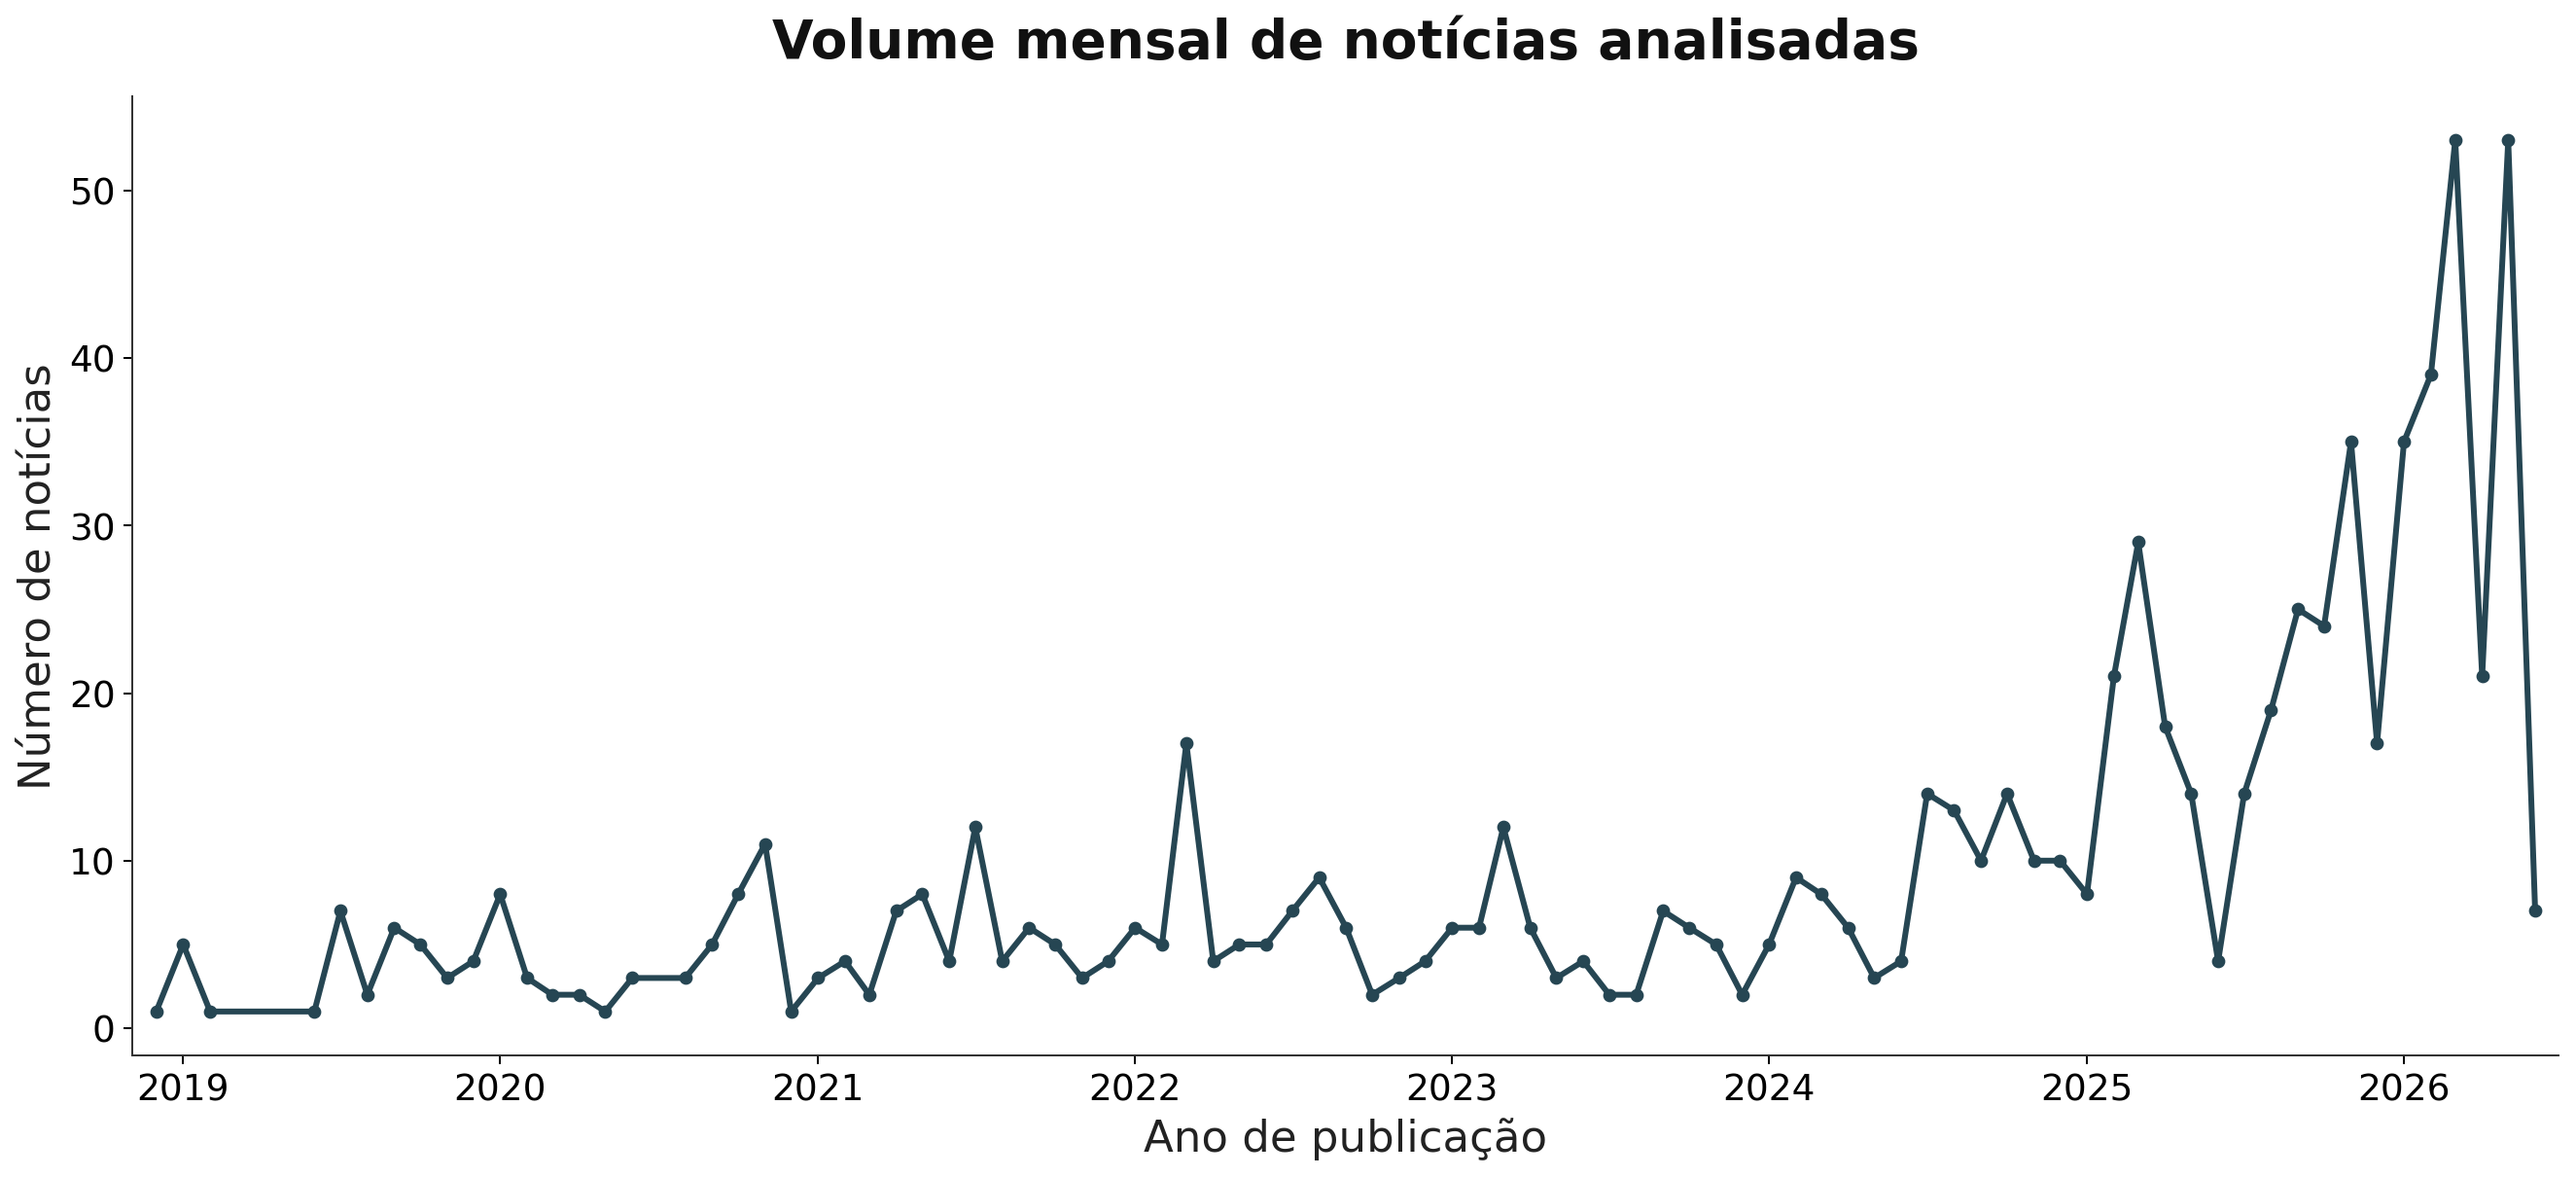
\includegraphics[width=0.95\textwidth]{graficos/linha_volume_mensal_noticias.png}
\caption{Volume mensal de notícias classificadas.}
\end{figure}

\subsection{Fontes}

\begin{figure}[H]
\centering
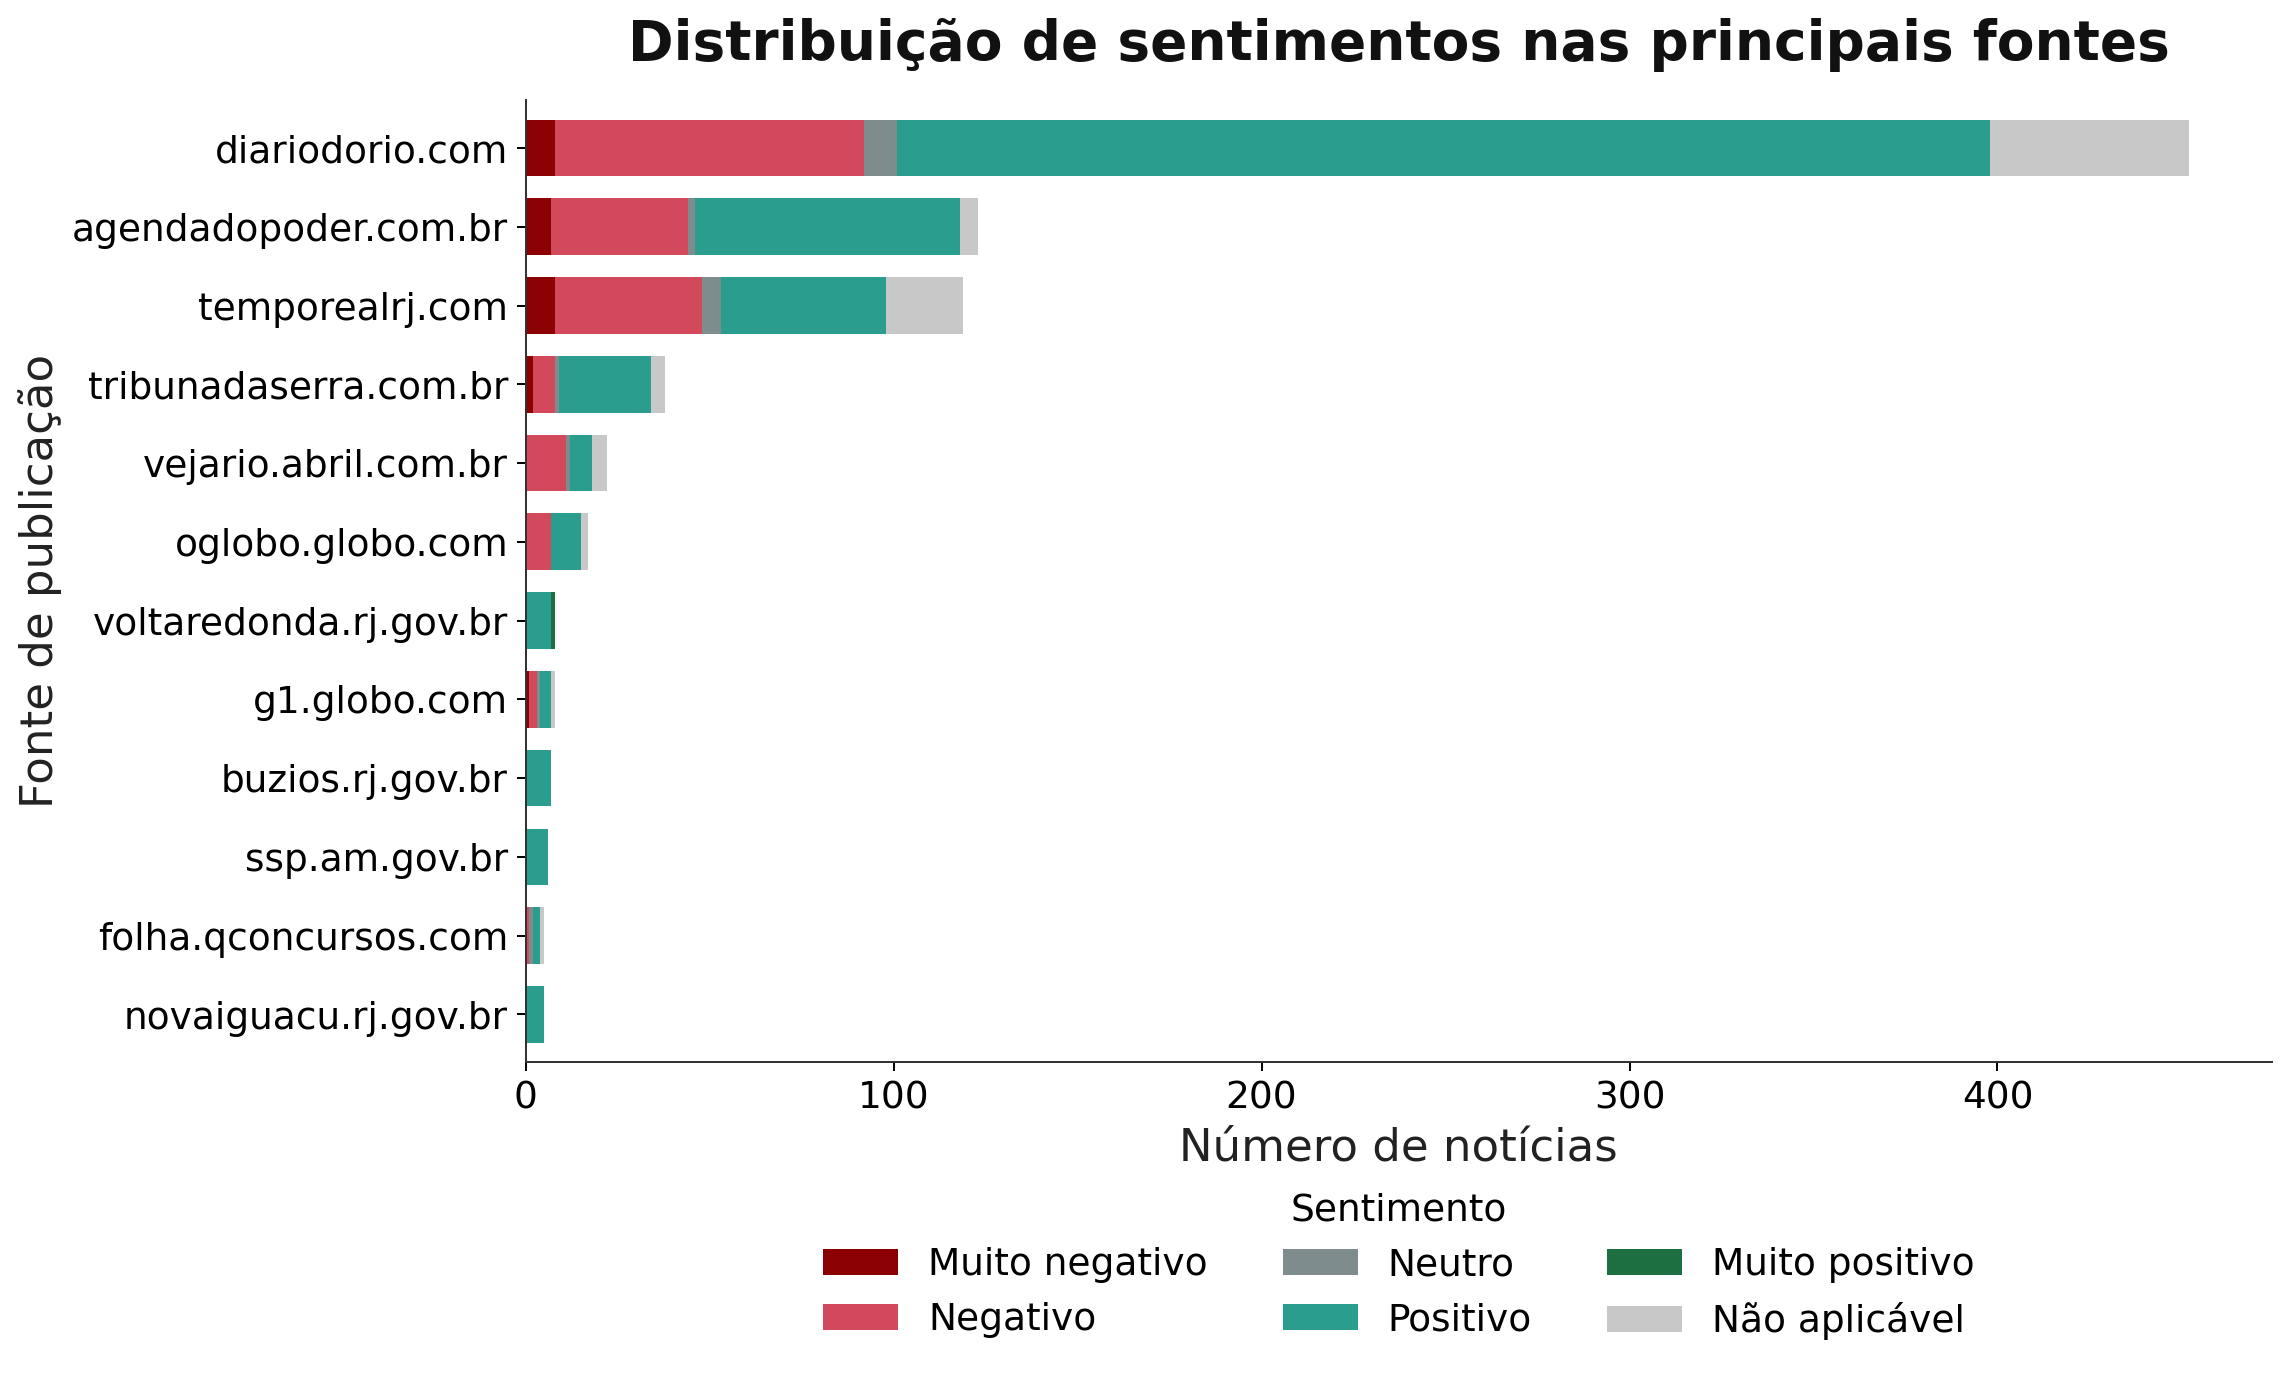
\includegraphics[width=0.95\textwidth]{graficos/barras_empilhadas_top_fontes.png}
\caption{Distribuição de sentimentos por fonte, considerando as principais fontes.}
\end{figure}

\section{Discussão}

% Os resultados apontam para uma cobertura predominantemente positiva do Segurança Presente no corpus analisado. Essa predominância está associada a notícias sobre expansão territorial, inauguração de bases, reforço de patrulhamento, operações em eventos públicos e ações administrativas apresentadas como ampliação da capacidade estatal. Em termos de enquadramento jornalístico, esses textos tendem a associar o programa a presença institucional, prevenção, ordenamento urbano e resposta operacional.

% Ao mesmo tempo, o corpus contém volume expressivo de notícias negativas. Essas notícias aparecem ligadas a controvérsias, críticas administrativas, problemas de gestão, eventos criminais com relação direta ou indireta ao programa, denúncias e situações em que a presença estatal é retratada como insuficiente, problemática ou politicamente contestada. A existência desse bloco negativo impede uma leitura simplista dos resultados: a predominância positiva não elimina tensões, disputas narrativas e episódios críticos.

% O ranking de eventos contribui para qualificar a interpretação. Enquanto a distribuição geral responde quantas notícias foram positivas ou negativas, o ranking permite identificar quais acontecimentos concretos concentraram elogios ou críticas. Essa mudança de escala é substantiva, porque notícias com linguagem parecida podem tratar de eventos diferentes, e notícias com títulos distintos podem se referir ao mesmo fato administrativo ou operacional.

\section{Conclusão}

% A pesquisa alcançou o objetivo de construir um procedimento automatizado para classificar notícias sobre o Segurança Presente, combinando análise de sentimento e extração de eventos factuais. A base final reuniu 847 notícias únicas, obtidas a partir de 863 registros coletados por webscrapping e filtradas por menção explícita ao programa. O método produziu uma leitura sistemática da cobertura entre 2016 e 2026, com predominância de notícias positivas, presença relevante de notícias negativas e identificação de eventos específicos associados a elogios e críticas.

% Do ponto de vista técnico, o principal ganho do procedimento está na integração entre classificação textual e estruturação analítica. O modelo de linguagem não foi usado apenas para atribuir rótulos; ele também extraiu eventos e justificativas, permitindo transformar uma coleção heterogênea de notícias em uma base passível de análise quantitativa e revisão qualitativa.

% Do ponto de vista substantivo, os resultados sugerem que o Segurança Presente aparece frequentemente associado a expansão, reforço operacional e presença institucional, mas também é atravessado por controvérsias administrativas, episódios negativos e disputas de interpretação.

\end{document}
